\chapter{Proposed solution}
\label{ch:proposed_solution}

In this particular paragraph we will deliberate the proposed model background and its main dissemblance from general unet architecture.

Jointly the solution it was utilized 2 convolution networks with same architectures but sundry purposes and parameters. By scenario firstly it is issued detection model afterwards identification model. The detection model comes up with segmenting of vertebra from background. Whereas the identification model identifies what vertebrates belong which segmented pixels. To fine it down the identification model does not categorize each pixel in discrete manner, vice continuously produce value which subsequently is rounded correspondingly to a specific vertebra. It worth to mention inwardly full solution captures both short-range and long range information. Short-range information is retrieved utilizing detection model. The identification model is trained by feeding in large slices which capture long-range information which is essential for the task of identifying individual vertebrae. Acquisition of final results is done by multiplying detection and identification models results to elaborate labels on each pixel afterwards aggregating them to produce final centroid estimates for each vertebra.

The step by step representation in terms of visualisation is demonstrated on the figure \ref{fig:detection_identification_steps}.

\begin{figure}[h]
    \centering 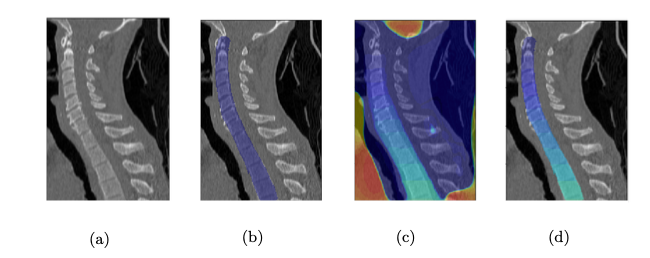
\includegraphics[width=9cm]{images/detection_identification_steps.png}
    \caption {(a) shows an original scan in grey-scale, (b) shows the output of the detection model applied to the scan, (c) shows the output of the identification model applied to the scan, (d) shows (b) and (c) multiplied together to produce a final prediction for each pixel.}
    \label{fig:detection_identification_steps}
\end{figure}

\section{Metrics}
\subsection{Dice score}
Recall the \cite{Thada2013} Dice similarity coefficient (Dice score) was used to quantify how closely identification predictions matched the training annotated ground truth segmentation. 

Assume we annotated some ground truth region in particular image and then make an automated algorithm to do it so far. To validate the algorithm it is calculated Dice score, which is a measure of how similar the objects are. In other words it is the size of the overlap of the two segmentations divided by the total size of the two objects. As for mathematical representation it is formed as:
\begin{align*}
  Dice score = \frac{2\cdot|A\cap B|}{2\cdot|A\cap B| + |B\backslash A| + |A\backslash B|}
\end{align*}

\subsection{ID rate}
It was introduced id rate measurement to validate correctness of closeness of predicted centroid estimations with ground truth vertebra centroid. 

\subsection{Localization error}
As for localisation error if centroid occurs at the scan it was deliberated by mean and std of distance of localization error between predicted centroid position and ground-truth centroid position for particular vertebrae. 


\section{Detection Model}
As previously mentioned detection model \ref{fig:detection_model} comes up with segmenting of vertebra from background. Taking it closer into consideration the model classifies each dedicated pixel of scan whether it is background or vertebrae. Jointly the initialization of weights it was  defined such as the background label with 0.1 weighting and the vertebrae label with 0.9 weighting. It was thought-out to repeal the fraction of nature background state at particular scan. As for loss function it was consumed \cite{Zhang2018} weighted categorical cross entropy with 2 classes, depicted as:
\begin{align*}
 L(P, Q) = 0.1 \cdot P(0)\log Q(0) + 0.9 \cdot P(1)\log Q(1)
\end{align*}
where P, Q - particular distributions 

Unlike standard unet architecture it was used same padding for all convolutional layers with stride 1, a learning rate
$\lambda$ of 0.001, a batch size of 16 and batch normalization after every convolutional layer with momentum of 0.1. The model implementation can be found in project repository.
\footnote{ \url{https://github.com/KumundzhievMaxim/VertebraeSegmentation/blob/main/train_detection_model.py}}

\begin{figure}[h]
    \centering 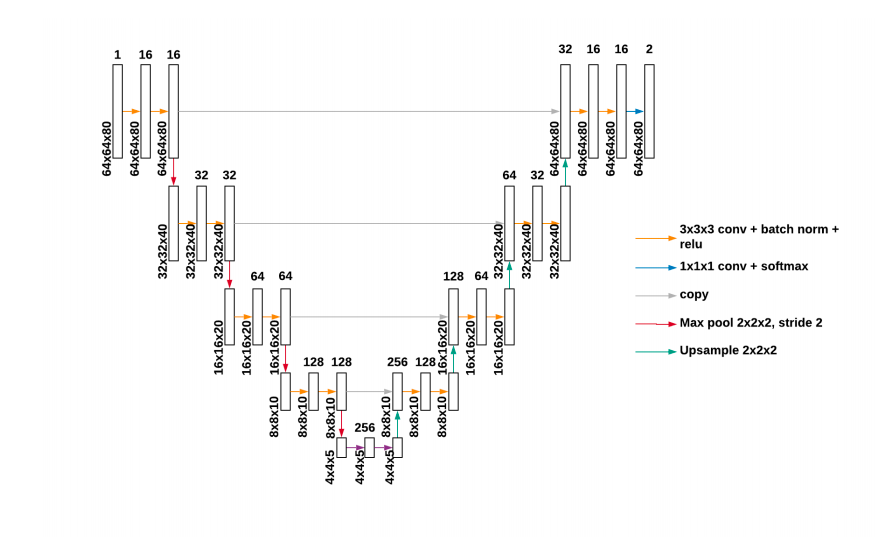
\includegraphics[width=9cm]{images/detection_model.png}
    \caption {Detection Model Architecture}
    \label{fig:detection_model}
\end{figure}
 
\subsection{Detection augmentation}
Unto passing particular batch of scans to detection model each image was represented as 5 cropped samples intruding that at least 4 of them contain some vertebrae pixels. In the meantime each sample scan was sized as $64 \cdot 64 \cdot 80$, meaning 64 pixels by 64 pixels by 80 channels. Withal accordingly each sample has an accompanying dense labelling, containing 0s (for background) and 1s (for vertebrae) of the same size.    
 
\section{Identification Model}
By the previous description identification model \ref{fig:identification_model} identifies what vertebrates belong which segmented pixels. For what it was established unet-wise architecture with revamped parameters. Updates brought changes of input layer channels number which corresponds to 8 to pass in samples of size $8 \cdot 80 \cdot 320$. The introduced filters sized $5 \cdot 20$ at the lowest level of the architecture  increases the size of the receptive field thereby maximizing the potential information retrieved by the network. To clarify, the background pixels are strained out, denoting just that pixels which are labeled as background when we train model. As for loss function the following modified L1 function was approached:
\begin{align*}
 L = \begin{cases} \lvert y_i - x_i \rvert\ \mbox{if } x\mbox{$\neq 0$} \\ 0, \mbox{ otherwise} \end{cases}
\end{align*}
where $y_i$ - predicted value of pixel $i$ and $x_i$ - true value of pixel $i$.
Unlike standard unet architecture it was used same padding for all convolutional layers with stride 1, a learning rate
$\lambda$ of 0.001, a batch size of 32 and batch normalization after every convolutional layer with momentum of 0.1. The model implementation can be found in project repository. \footnote{\url{https://github.com/KumundzhievMaxim/VertebraeSegmentation/blob/main/train_identification_model.py}}

\begin{figure}[h]
    \centering 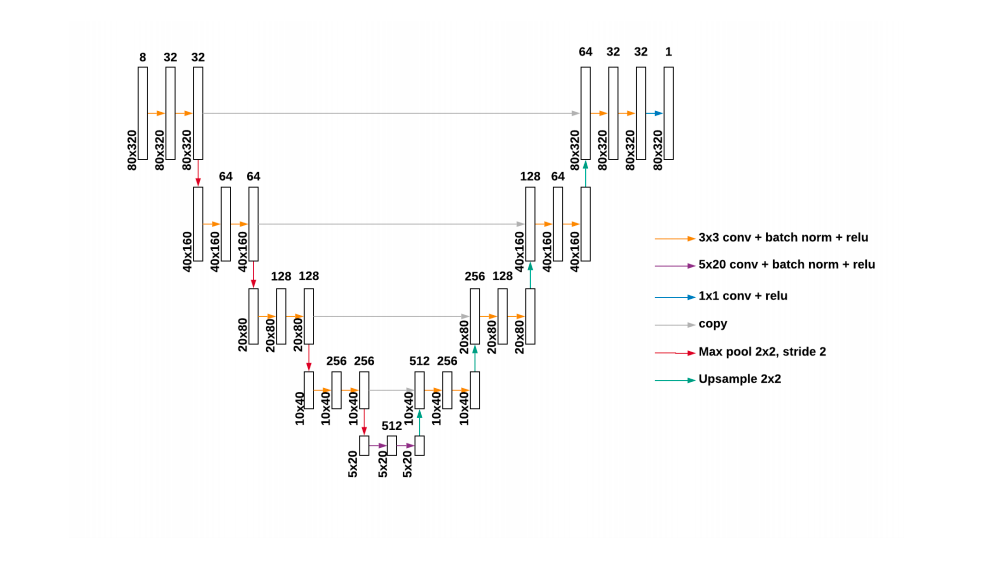
\includegraphics[width=9cm]{images/identification_model.png}
    \caption {Identification Model Architecture}
    \label{fig:identification_model}
\end{figure}

The identification model outputs a continuous value for each pixel of a scan which, is rounded to an integer to correspond to a specific vertebrae. The identification model gives a value to each pixel even if that pixel is not depicting any vertebrae and is a background. These pixels will be filtered out of the final predictions by multiplying them by their corresponding pixel from the output of the detection model which should be 0 for a background pixel. The model outputs are represented as continuous value for each dedicated pixel of particular scan which further is rounded to correspond to a specific vertebrae integer. As well it should be considered the model award each pixel's value nay it is background and does not represent any vertebrae. Even though these pixels will be filtered out of the final predictions by multiplying them by their corresponding pixel from the output of the detection model which should be 0 for a background pixel.

\subsection{Identification augmentation}
Altogether proceeding with identification network for each scan in the training set it was produced 100 cropped samples sized $8 \cdot 80 \cdot 320$ coercing all of them retrieving some vertebrae pixels whereas each with a corresponding dense labelling of size $80 \cdot 320$, representing the labelling for the forth slice of the input sample.

\section{Inference}
As soon as the identification model outcomes predicted label per each pixel foremost thresholding $x_\upsilon$ is applied as validation whether include particular centroid in the prediction or not by comparing the obtained  number of pixels for a vertebra and assumed thresholding number.

The threshold $x_\upsilon$ is specific to the vertebra $\upsilon$ and formed as:
\begin{align*}
  x_\upsilon = \max(3000, 0.4 \cdot R_\upsilon^3) 
\end{align*}
where R - the radius of the vertebra $v$
